Bitcoin was not created in a vacuum and to understand the design of Bitcoin and by extension the Lightning Network one would
benefit from understanding money and systems of trust. Nakamoto encoded "the times 03/jan/2009 chancellor on brink of second bailout for banks"\cite{repository:bitcoin:sourceforge}\cite{bitcoin:genesis:coinbase} in coinbase transaction of the genesis block as an alleged comment on the current banking system as well as a time stamp. He later cemented this view with multiple forum posts while he still was active.

\subsection{Origin of money}

On the fringes of our specie barter became the first
medium of which made trade viable, removing the risk 
from otherwise simple delayed reciprocity. It is possible
for a trade to be mutual beneficial as Nick Szabo 
se elegantly explained:

\begin{displayquote}
"individuals, clans, and tribes all vary in their preferences, vary in their ability to satisfy these preferences, and vary in the beliefs they have about these skills and preferences and the objects that are consequent of them, there are always gains to be made from trade."\cite{szabo:shelling:out}
\end{displayquote}

Barter is by itself quite limiting, consider a \textit{System S}
consisting of \textit{n} commodities, the amount of possible exchanges
between commodities in \textit{S} is \textit{n x n}. When n increases, the exchange pairs increases exponentially,
taxing the mind and decrease the coincidence of trade\footnote{The coincidence of finding another party who is looking to exchange the same commoditiy pair but in opposite order.}. 
The economist Carl Menger described it as inevitable for money to evolve from a sufficient volume of
commodity barter\cite{menger:origins:money}. If the same System S is considered with money - the possible exchange pairs would be reduced to only \textit{n} pairs. 

\subsubsection{Properties of money}

\subsection{Bearer promissory notes}

Although gold emerged as the commodity best suited as money
it still had two major problems:

\begin{enumerate}
	\item It's unsuitable for small transactions due to the limit in divisibility.
	\item It's expensive to carry around and protect.
\end{enumerate}

Private banks started to issue bearer promissory notes to the owners of the underlying asset it stored(e.g figure \ref{fig:seb:promissory:note}). 
The asset could then be retrieved for the note on demand. The notes themselves could then be traded 
instead of the underlying gold. This solved both the above problems, notes are easy to carry, conceal and 
could be minted in very small amounts. 

\begin{figure}[!htb]
	\centering
	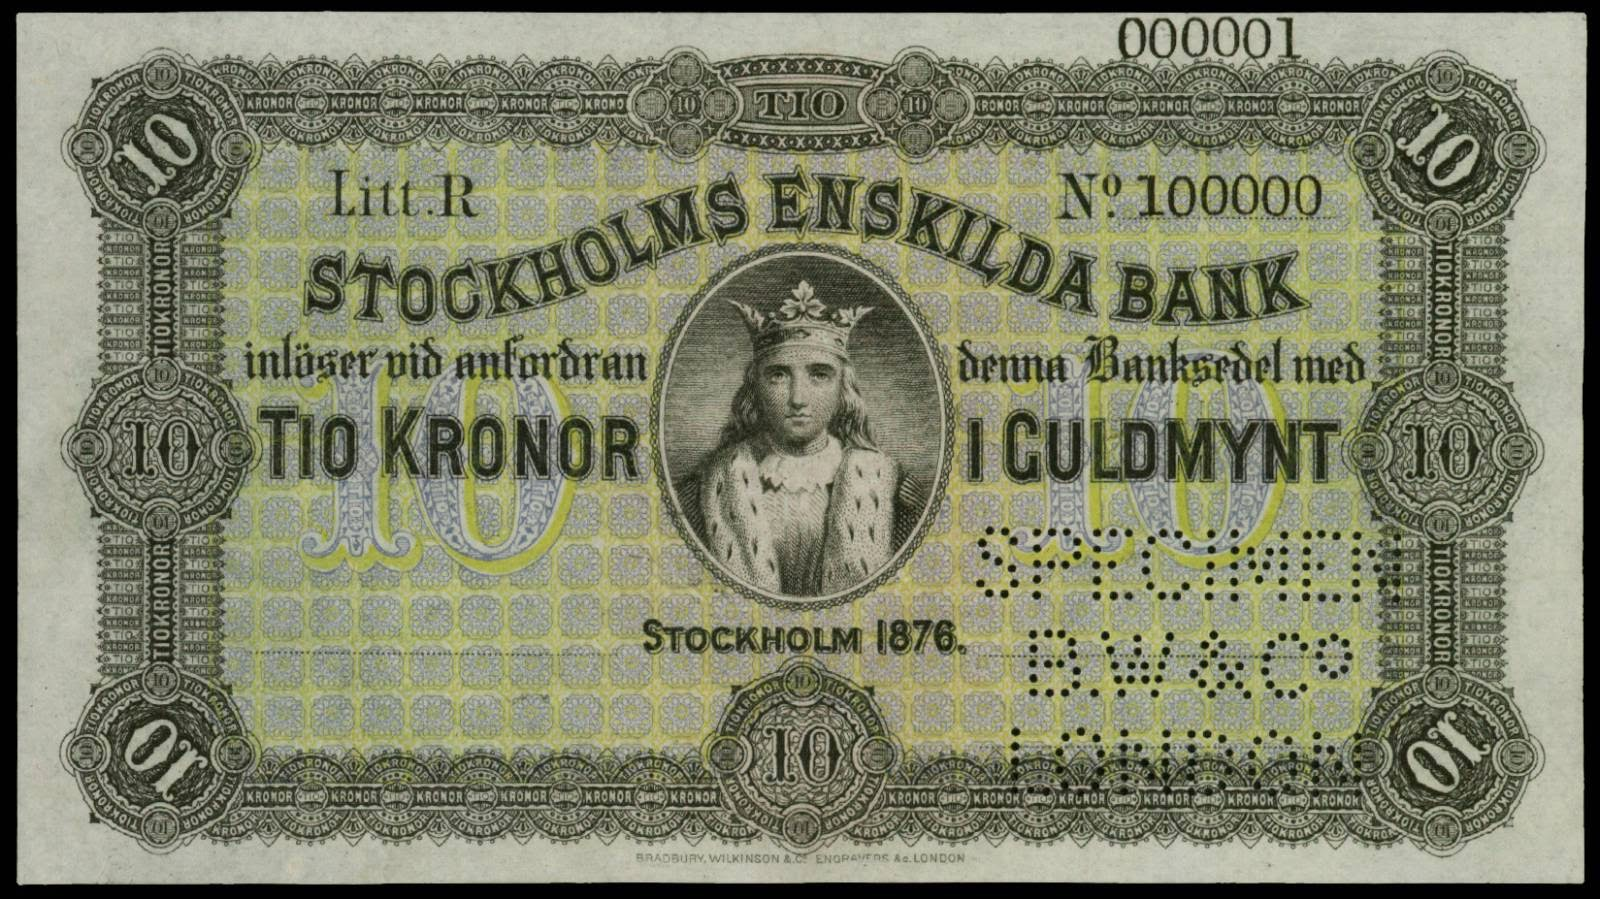
\includegraphics[width=7cm]{PrivateBankNoteStockholmEnskildaBank1876.JPG}
	\caption{\textit{The private bank 'Stockholms Enskilda Bank'(SEB) issued bearer
	promissory note. It promises to pay 10 crowns to the bearer upon demand in gold. 
	The exchange rate as per the Scandinavian Convention(Sweden, Denmark 27 may 1873, Norway 1 april 1877)\cite{nordic:crown}
	was 1 kilogram gold per 2480 crowns or 1 crown per 0.403g gold\cite{crown:gold}. 
 }}
	\label{fig:seb:promissory:note}
\end{figure}

By the late 19th century almost all currency was redeemable for gold.[?]

\subsubsection{Bank runs}

The introduction of the promissory note solved the two previously mentioned problems but also 
introduced trust. 
  






in the 1800 hundreds gold was 

\subsection{Elastic money}
\subsection{Relevancy}
In many ways it help to think of bitcoin
as both a bearer instrument and as a monetary system and how the 
system is designed as such. This
section is an incomplete view on it's own and
further reading is encouraged: 

* Nick Szabo's Enumerated 
